\documentclass[10pt,a4paper,notitlepage]{article}
\usepackage[utf8]{inputenc}
\usepackage{amsmath}
\usepackage{amsfonts}
\usepackage{amssymb}
\usepackage{mathtools}
\usepackage{fullpage}
\usepackage{lastpage}
\usepackage{fancyhdr}
\usepackage{fancyvrb}
\usepackage{graphicx}
\graphicspath{{./Graphics/}}
\usepackage{float}
\usepackage{nameref}
\author{Jonah Gibbon}
\usepackage[backend=bibtex,style=authortitle-ibid]{biblatex}
\addbibresource{References.bib}


\pagestyle{fancy}
\fancyhf{}
\renewcommand{\headrulewidth}{0pt}
\cfoot{Page \thepage\ of \pageref{LastPage}}

\newcommand{\abs}[1]{\lvert#1\rvert}
\newcommand{\Z}{\mathbb{Z}}
\newcommand{\Q}{\mathbb{Q}}
\newcommand{\C}{\mathbb{C}}
\newcommand{\N}{\mathbb{N}}
\newcommand{\R}{\mathbb{R}}
\newcommand{\Nd}{\mathcal{N}}
\newcommand{\Var}[1]{\mathrm{Var}\left(#1\right)}
\newcommand{\E}[1]{\mathbb{E}\left(#1\right)}
\newcommand{\p}[1]{\mathbb{P}\left( #1 \right)}

\begin{document}
\subsection*{\centering Question 1}\label{sec:Q1}
Integrating to find the median gives
\begin{equation}
\int_{0}^{m}\theta e^{-\theta x}\mathrm{d}x=\left[-e^{-\theta x}\right]^{m}_{0}=1-e^{-\theta m}=1/2
\end{equation}
Therefore $\theta= \log(2)/m$ and $g(x\, |\, m)= \log(2)/(m\cdot 2^{x/m})$.
\subsection*{\centering Question 2}\label{sec:Q2}
The program \nameref{cd:2.1}, referenced on page \pageref{cd:2.1}, produced the exponential random variables $x_{i}$ from the uniform random variables $u_{i}$ in Table \ref{tb:Q2}. It also plotted the log likelihood function in Figure \ref{fig:Q2} using the same data. 
\begin{table}[H]
\centering
\begin{tabular}{|c|c|c|}\hline $i$ & $u_{i}$ & $x_{i}$\\ \hline 1 & 0.15237801896922 & 0.1377670997206\\ 2 & 0.82581697748955 & 1.4563738992246\\ 3 & 0.53834243526006 & 0.64410988715659\\ 4 & 0.99613471662689 & 4.6297669015646\\ 5 & 0.078175528753184 & 0.067833709839194\\ 6 & 0.44267826977545 & 0.48717716099783 \\ \hline \end{tabular}
\caption{Exponential Variables with $n=6$ and $\theta_{0}=1.2$}
\label{tb:Q2}
\end{table}
\begin{figure}[H]
\begin{center}
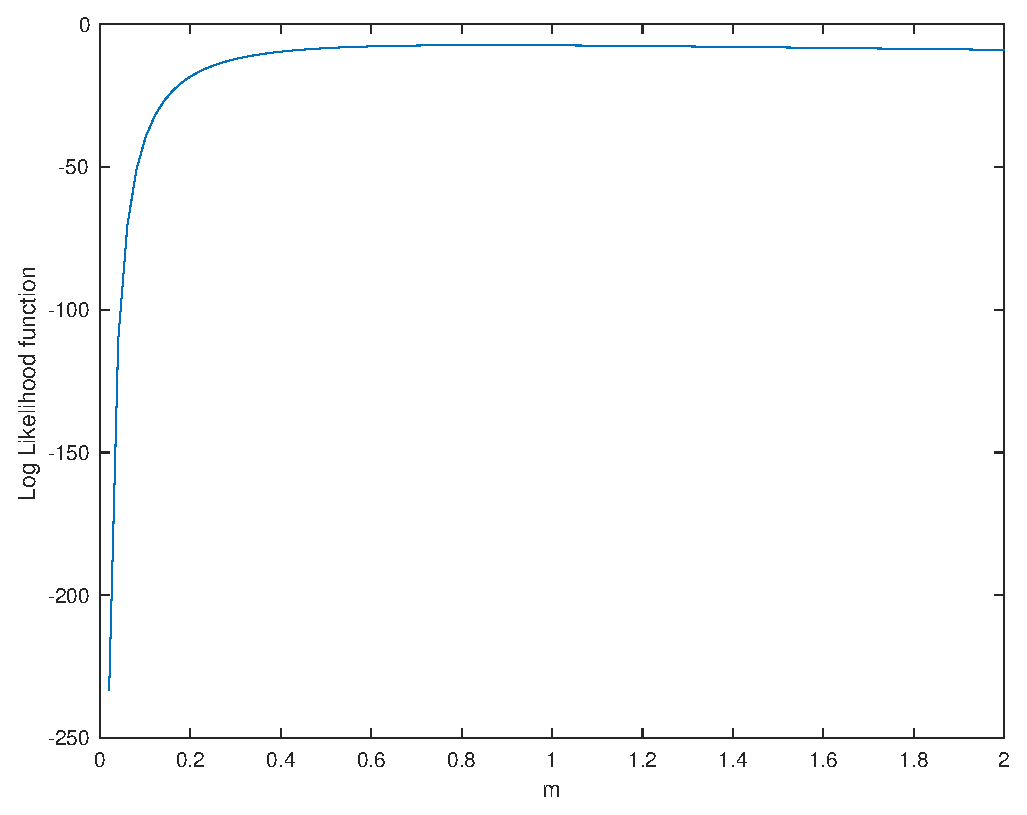
\includegraphics[width=10cm]{Image_3_1}
\caption{Plot of the log likelihood function against $m$ with $n=6$}
\label{fig:Q2}
\end{center}
\end{figure}

Expanding $\ell_{n}(m)$ gives
\begin{equation}\label{eq:ELL}
\ell_{n}(m)=n\log\left(\log\left(2\right)\right)-n\log\left(m \right)-\frac{\log\left(2\right)S}{m}
\end{equation}
where $S=\sum_{i}x_{i}$. Differentiating with respect to $m$ gives the maximum value $\widehat{m}_{n}=\log(2)\sum_{i}x_{i}/n$.  (This is indeed a maximum since $\ell_{n}$ is continuous, and it's endpoints $\left(0,\infty\right)$ tend to $-\infty$. Therefore the maximum must occur at the only turning point). For the example given above, we calculate $\widehat{m}_{6}$ as 0.857541897642894, which is not a good approximation to the actual value $m_{0}=0.5776226505$. This is because the variance in $\widehat{m}_{n}$ is 
\begin{equation}
\frac{\log(2)^2}{n^2} \sum_{i=1}^{n}\Var{x_{i}}=\frac{\log(2)^2}{n}\times \frac{1}{\theta^2}=\frac{m_{0}^2}{n}
\end{equation}
and so when $n$ is small, this value is likely not to be accurate. However as $n\rightarrow \infty$ this variance will tend to 0, and so $\widehat{m}_{n}\rightarrow \E{\widehat{m}_{n}}=\log(2)/\theta_{0}=m_{0}$.\footnote{Note that the same result can also be proved using the law of large numbers.} We deduce further that this maximum likelihood estimator is unbiased.

\subsection*{\centering Question 3}

\nameref{cd:2.1} was also used to produce Figure \ref{fg:3.1}, a plot of the log likelihood function for different values of $n$.
\begin{figure}[H]
\begin{center}
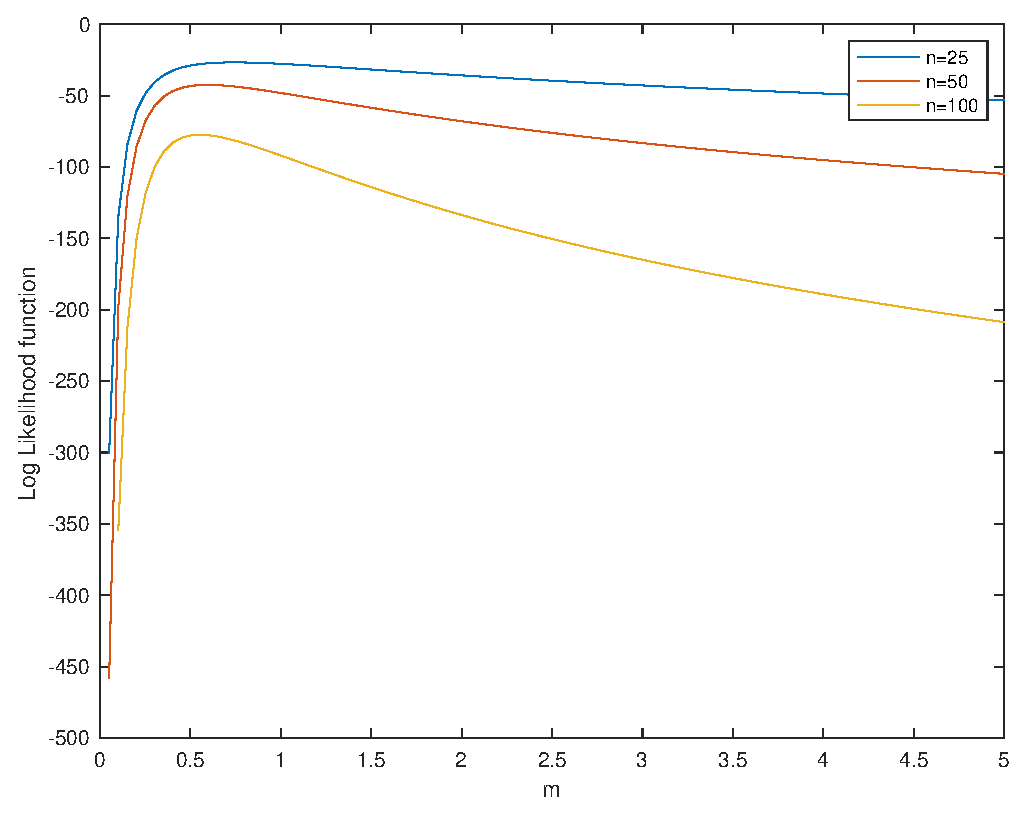
\includegraphics[width=10cm]{Image_3_2}
\caption{Plot of the log likelihood function against $m$ with different $n$}
\label{fg:3.1}
\end{center}
\end{figure}
\begin{table}[H]
\centering
\begin{tabular}{|c|c|}
\hline $n$ & $\widehat{m}_{n}$ \\ \hline 
25 & 0.73960458432 \\
50 & 0.59504738029 \\
100 & 0.55249375490 \\ \hline
True Value $m_{0}$ & 0.5776226505 \\ \hline
\end{tabular}
\caption{$\widehat{m}_{n}$ for data in Figure \ref{fg:3.1}}\label{tb:Q3}
\end{table}

Firstly note that Table \ref{tb:Q3} confirms the idea that $\widehat{m}_{n}\rightarrow m_{0}$. We also observe that as $n$ increases, the hight of each maximum is decreasing. The value of the log likelihood function at its maximum is
\begin{equation}
-n\left(1+\log\left(\frac{S}{n}\right)\right)
\end{equation}
By the law of large numbers, when $n$ is big we may consider $S/n\approx 1/\theta_{0}$. So for $\theta_{0} < e$ the maximums will decreases, and for $\theta_{0}>e$ the maximums will increase. Certainly when $\theta_{0}=1.2$ the values of the maximums are decreasing. \par
We can see that $\ell_{n}\left(m\right)$ tends to $-\infty$ as $\theta$ grows very small. This makes sense, since $f(x,\, |\, m=0)=0$ and so taking the logarithm means this will occur for any values of $x_{i}$. Notice that as $n$ increases, the log-likelihood function decays faster. This is because when $m$ is large, $\ell_{n}(m)\approx -n\log(m)$, and so visibly decays quicker.

\subsection*{\centering Question 4}

Expanding $M_{X}(\lambda)$ gives
\begin{equation}
\E{e^{\lambda X}}=\int_{0}^{\infty}e^{\lambda x}f\left(x|\theta\right)\mathrm{d}x=\theta\int_{0}^{\infty}e^{(\lambda-\theta) x}\mathrm{d}x=\frac{\theta}{\lambda-\theta}\left[e^{(\lambda-\theta)x}\right]_{0}^{\infty}
\end{equation}
Therefore $M_{X}(\lambda)$ equals $\theta/(\lambda-\theta)$ for $\lambda<\theta$ and does not exist for $\lambda\geq \theta$.\\

For the second part we will aim to prove a stronger statement; if $X \sim \Gamma(p,\theta)$ and $Y\sim\Gamma(q,\theta)$ are independent, then $X+Y\sim\Gamma(p+q,\theta)$. The moment generating function $M_{X+Y}\left(t\right)$ is equal to $\E{\exp\left(t(X+Y)\right)}=\E{\exp\left(tX\right)}\E{\left(tY\right)}$ (since independent) $= \left(1-t/\theta\right)^{-(p+q)} = M_{Z}\left(t\right)$ where $Z\sim\Gamma\left(p+q,\theta\right)$. We now use the fact that if two random variables have the same moment generating function in some non-zero interval around 0 then they are identically distributed.\footnote{The proof of this is laid out in \cite{TheoryMG}} We are therefore done, since these moment generating functions are identical in the interval $t\in[-\theta/2,\theta/2]$. In the case of Question 4, notice that the exponential distribution is identical to a $\Gamma\left(1,\theta\right)$ distribution, and so the result follows immediately. 

\subsection*{\centering Question 5}
Integrating by parts twice gives
\begin{equation}\label{eq:6}
F(x)=\int^{x}_{0}\theta^{2}t e^{-\theta t}\mathrm{d}t=\theta^{2}\left[-\frac{te^{-\theta t}}{\theta}-\frac{e^{-\theta t}}{\theta^{2}}\right]^{x}_{0}=1-(\theta x+1)e^{-\theta x}
\end{equation}
Let $\omega = -\theta x-1$, so if $F(x)=k$, then $(k-1)/e=\omega e^{\omega}$, or $\omega=W\left(\frac{k-1}{e}\right)$, where $W$ represents the Lambert W function. Assume that we could solve for $x$ in closed form. This would imply we could solve for $\omega$, and hence $W$, in closed form too. However we know that the Lambert W function cannot be solved in closed form, and so we conclude that neither can $x$.\footnote{The proof that the Lambert W function cannot be written in closed form is laid out in \cite{Rosenlight1969}.}

\subsection*{\centering Question 6}
The log likelihood function is now equal to
\begin{equation}\label{eq:LLFConcave}
\ell_{n}=\log\left( \theta^{2n}e^{-\theta S}\cdot\prod_{i=1}^{n}x_{i}\right)=2n\log(\theta)-\theta S+\sum_{i=1}^{n}\log(x_{i})
\end{equation}
Differentiating with respect to $\theta$ gives
\begin{equation}
0 = \frac{\mathrm{d}\ell_{n}}{\mathrm{d}\theta}=\frac{2n}{\widehat{\theta}_{n}}-S
\end{equation}
or that a maximum occurs at $\widehat{\theta}_{n} = 2n/S$ (where $S$ is the same as in Question 2). This is indeed a maximum since $\ell_{n}\left(\theta\right)\rightarrow -\infty$ at $\theta=0,\infty$. By the law of large numbers, for large $n$, $S/n\rightarrow \E{X}$ (where $X$ has p.d.f $f(x\, |\, \theta)$). $\E{X}=\left[ (-\theta x^{2}-2x-2/\theta)e^{-\theta x}\right]_{0}^{\infty}=2/\theta_{0}$, and so $\widehat{\theta}_{n}\rightarrow \theta_{0}$.
\subsection*{\centering Question 7}
The program \nameref{cd:7.1}, referenced on page \pageref{cd:7.1}, was used to produce Figure \ref{fg:7.1} and the maximum likelihood estimators in Table \ref{tb:Q7}.
\begin{figure}[H]
\centering
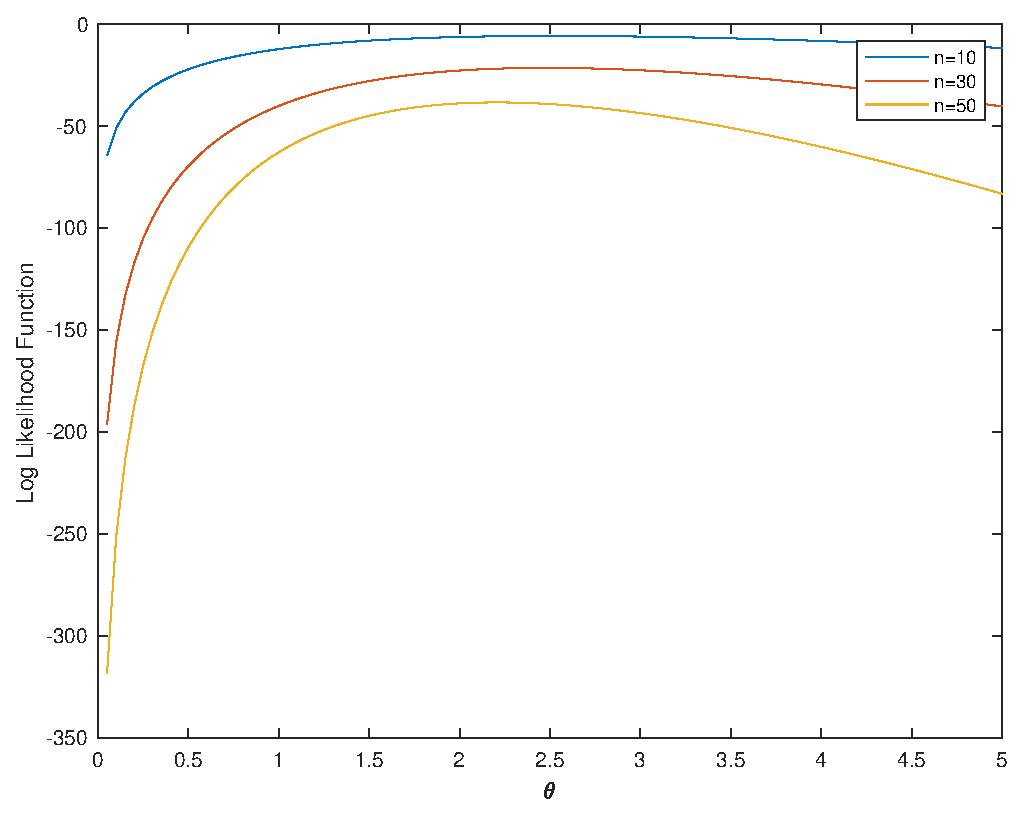
\includegraphics[width=10cm]{Image_7_1}
\caption{$\ell_{n}(\theta)$ against $\theta$ with $n=10,30$ and $50$}\label{fg:7.1}
\end{figure}
\begin{table}[H]
\centering
\begin{tabular}{|c|c|}
\hline $n$ & $\widehat{\theta}_{n}$ \\ \hline 10 & 2.52903145291339 \\ 30 & 2.4787073067176 \\ 50 & 2.20599743507643 \\ \hline Actual Value $\theta_{0}$ & 2.2 \\ \hline
\end{tabular}
\caption{$\widehat{\theta}_{n}$ for data in Figure \ref{fg:7.1}}
\label{tb:Q7}
\end{table}
Firstly we can verify that the m.l.e. tends towards $\theta_{0}$. Secondly in Figure \ref{fg:7.1} the log likelihood function appears strictly concave, whereas in Figure \ref{fg:3.1} this is not the case. We deduce from equation \eqref{eq:LLFConcave} that $\ell_{n}''=-2n/\theta^{2}<0$ for all $\theta$.\footnote{Here $\ell_{n}''$ represents the second derivative of the log likelihood function with respect to $\theta$.} What's interesting about this is that no matter the values of $x_{i}$, $\ell_{n}$ will always be strictly concave, unlike the first case where it is only strictly concave in the region $(0,\log(4)S/n)$.  

Another difference is that $\ell_{n}\left(\theta\right)$ decays constantly with gradient $-S$ as $\theta\rightarrow\infty$, unlike the $-n\log\left(m\right)$ decay seen in Figure \ref{fg:3.1}. We can still see $\ell_{n}$ tending to $-\infty$ for large and small $\theta$. This is similar to Figure \ref{fg:3.1}, and still would be the case if we parametrised $\ell_{n}$ in terms of $m$. This is because from equation \eqref{eq:6} we can deduce that $\theta m=K$ for some constant $K$. Therefore if $\theta\rightarrow \infty$, $m\rightarrow 0$, and likewise the other way around, so this property is preserved when parametrising in terms of $\theta$ or $m$.

\subsection*{\centering Question 8}
We can analyticity derive the p.d.f. for $\widehat{\theta}_{n}=2n/\sum_{i} x_{i}$. We know each $x_{i}\sim \Gamma\left(2,\theta\right)$, so $\widehat{\theta}_{n}\sim 2n/Y$ where $Y\sim \Gamma\left(2n,\theta\right)$ (using Question 4). Defining the 1-1 function $Z=g\left(Y\right)=2n/Y$ means the p.d.f. of $Z$, $f_{Z}\left(y\right)$ is
\begin{equation}\label{eq:Q8PDF}
\begin{aligned}
f_{Z}\left(y\right) &= f_{Y}\left(g^{-1}\left(y\right)\right)\left| \frac{\mathrm{d}}{\mathrm{d}y}g^{-1}\left(y\right)\right|\\
&= \frac{\theta^{2n}}{\Gamma\left(2n\right)}\left(\frac{2n}{y}\right)^{2n-1}\exp\left(\frac{-2n\theta}{y}\right)\times\frac{2n}{y^2}\\
&=\frac{\left(2n\theta\right)^{2n}}{\Gamma\left(2n\right)y^{2n+1}}\exp\left(\frac{-2n\theta}{y}\right)
\end{aligned}
\end{equation}
\nameref{cd:8.1}, referenced on page \pageref{cd:8.1}, was used to produce Figures \ref{fg:8.1} to \ref{fg:8.2} to investigate the distribution of $\widehat{\theta}_{n}$. (The exact p.d.f was superimposed, along with the true value $\theta_{0}$).
\begin{figure}[H]
\centering
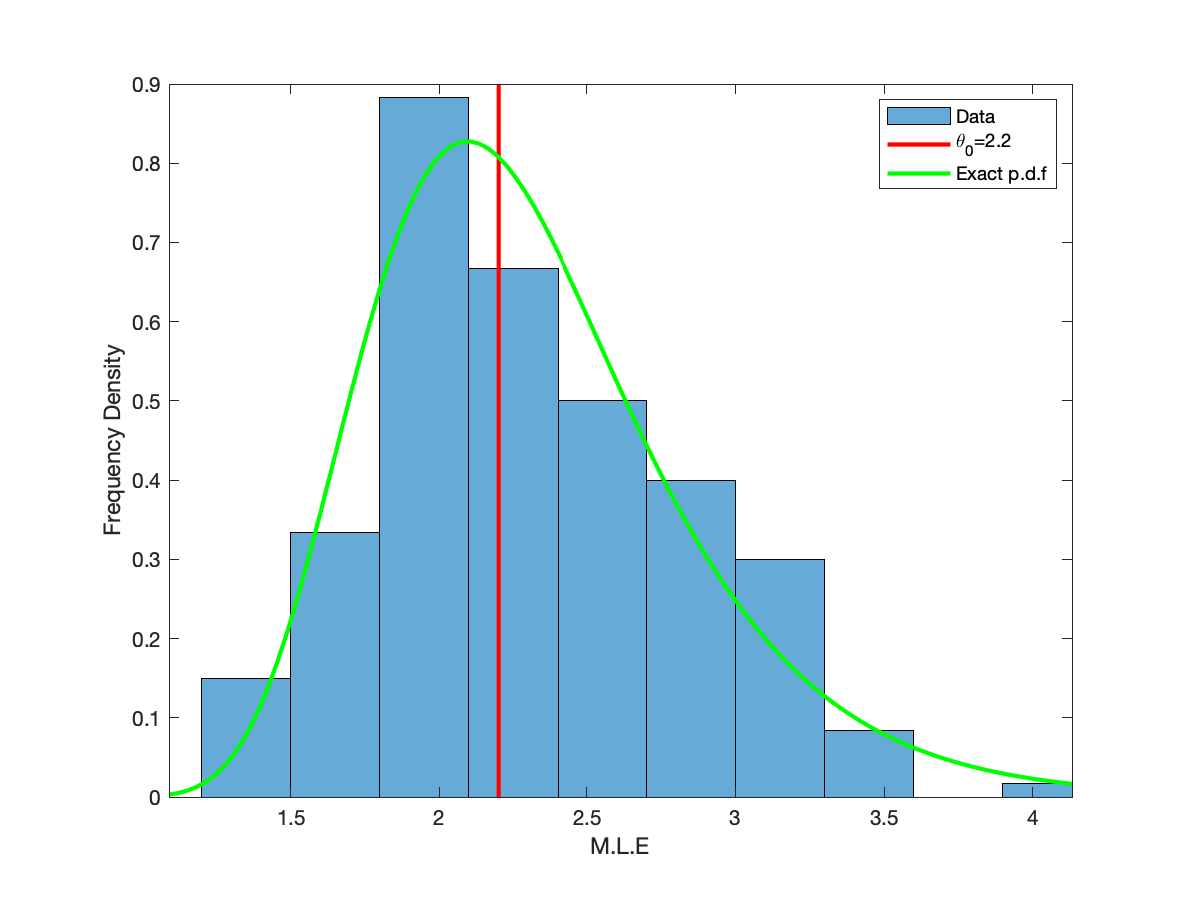
\includegraphics[width=10cm]{Image_8_1}
\caption{P.d.f. of m.l.e with $n=10$}\label{fg:8.1}
\end{figure}
\begin{figure}[H]
\centering
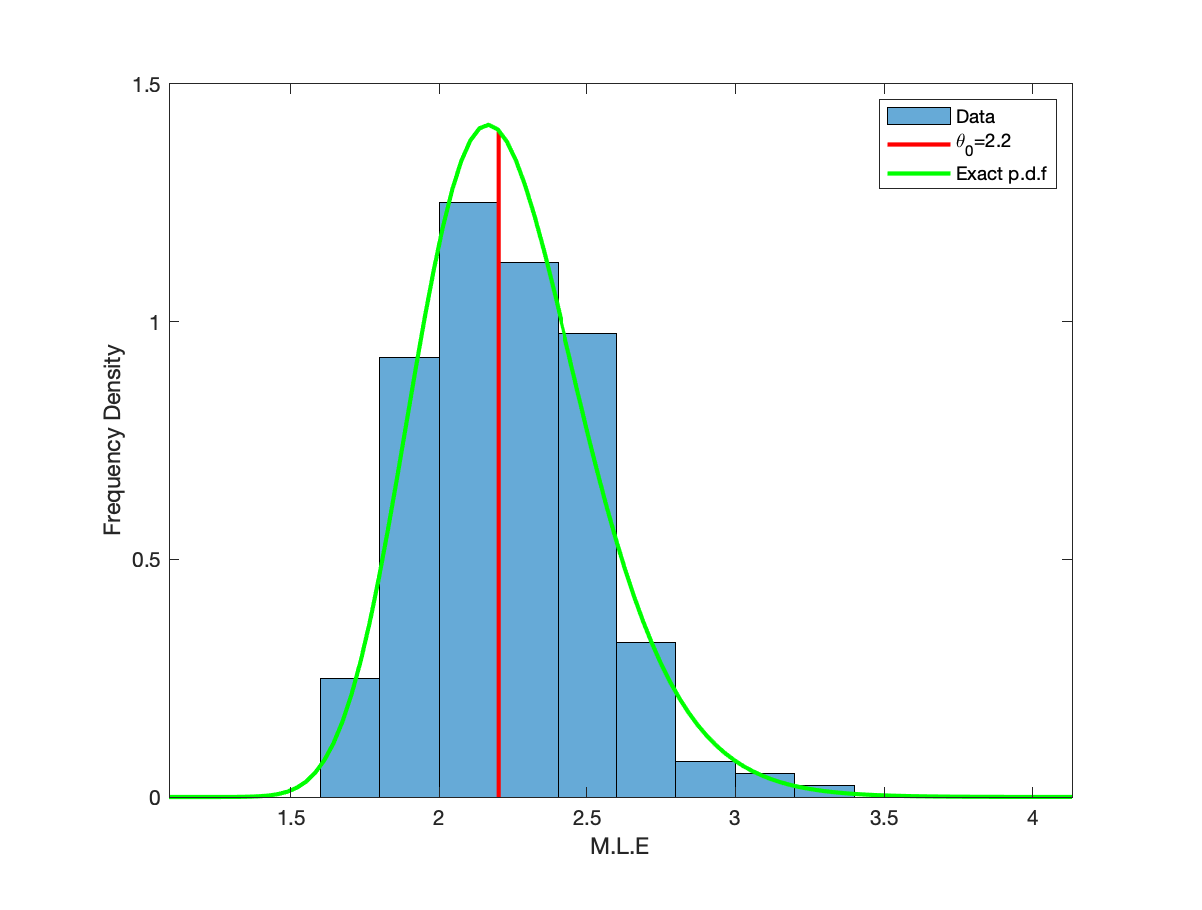
\includegraphics[width=10cm]{Image_8_2}
\caption{P.d.f. of m.l.e with $n=30$}
\end{figure}
\begin{figure}[H]
\centering
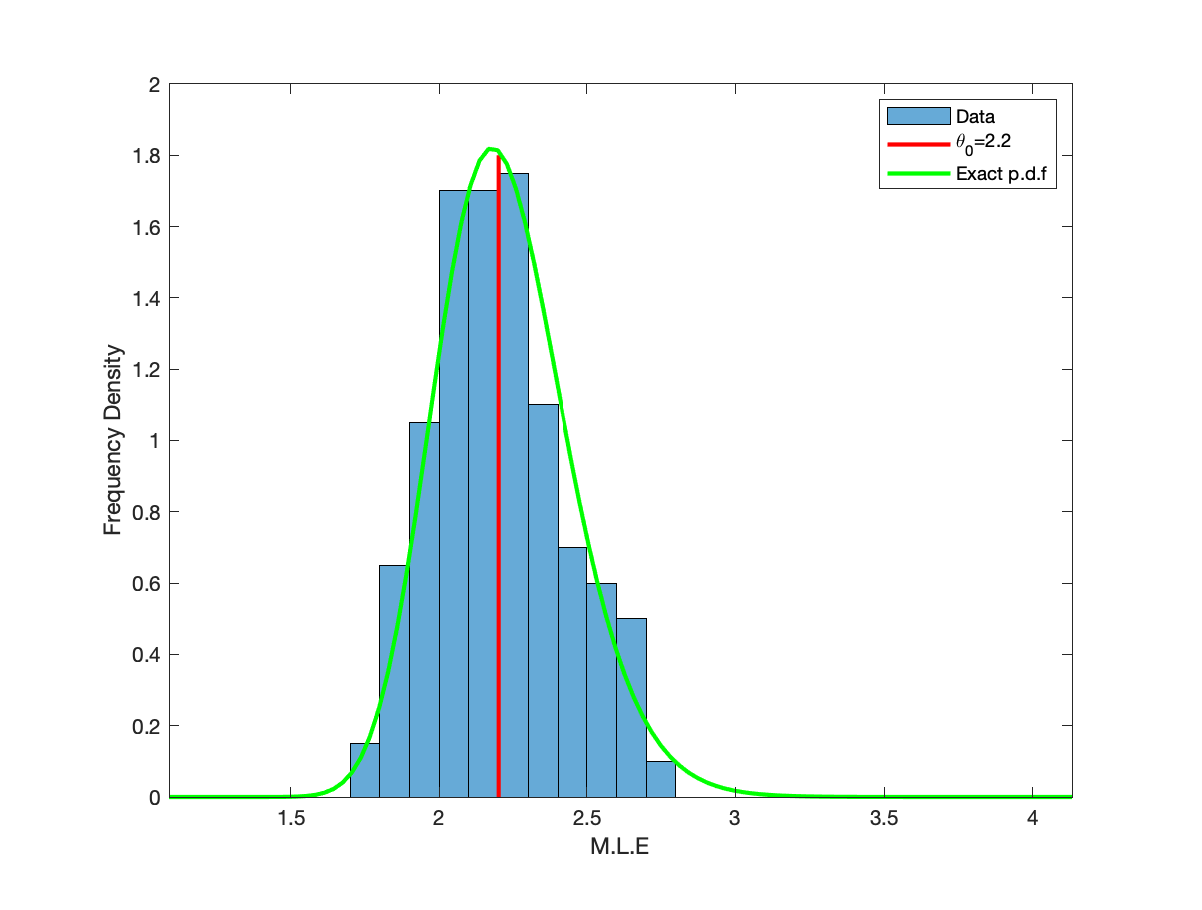
\includegraphics[width=10cm]{Image_8_3}
\caption{P.d.f. of m.l.e with $n=50$}\label{fg:8.2}
\end{figure}

\begin{table}[H]
\centering
\begin{tabular}{|c|c|c|}
\hline $n$ & Average m.l.e & Variance from $\theta_{0}$ \\ \hline 10 & 2.31165782061807 & 0.27443154548354\\ 30 & 2.23204239273873 & 0.0864587928435113 \\ 50 & 2.20292403340839 & 0.0482363078542326\\ \hline 
\end{tabular}
\caption{Average and Variance in Histogram Data}
\label{tb:Q8}
\end{table}
Firstly note that these histograms are approximations of the p.d.f. for $\widehat{\theta}_{n}$, as they plot the (sampled) frequency density.\footnote{These histograms have been normalised so that they match with the exact p.d.f.} Observe that as $n$ increases, it appears the variance from $\theta_{0}$ shrinks to 0 and the expectation tends to $\theta_{0}$. We hypothesis that
the p.d.f $f_{Z}(y)$ approaches $\delta(y-\theta_{0})$ for large $n$ ( $\delta$ represents the Dirac delta function). To better understand how $\widehat{\theta}_{n}$ behaves, we can calculate the exact expectation and variance using equation \eqref{eq:Q8PDF}:
\begin{equation}
\begin{aligned}
\E{\widehat{\theta}_{n}} &=\frac{\left(2n\theta\right)^{2n}}{\Gamma\left(2n\right)}\int_{0}^{\infty}\frac{y}{y^{2n+1}}\exp\left(\frac{-2n\theta}{y}\right)\mathrm{d}y\\
&= \frac{2n\Gamma\left(2n-1\right)}{\Gamma\left(2n\right)}\theta_{0}\\
&=\frac{2n\theta_{0}}{2n-1}
\end{aligned}
\end{equation}
and
\begin{equation}
\begin{aligned}
\Var{\widehat{\theta}_{n}} &=\frac{\left(2n\theta\right)^{2n}}{\Gamma\left(2n\right)}\int_{0}^{\infty}\frac{y^{2}}{y^{2n+1}}\exp\left(\frac{-2n\theta}{y}\right)\mathrm{d}y-\left(\frac{2n\theta_{0}}{2n-1}\right)^{2}\\
&= \frac{4n^{2}\Gamma\left(2n-2\right)\theta_{0}^{2}}{\Gamma\left(2n\right)}-\left(\frac{2n\theta_{0}}{2n-1}\right)^{2}\\
&= \frac{4n^{2}\theta_{0}^{2}}{\left(2n-1\right)^{2}\left(2n-2\right)}
\end{aligned}
\end{equation}
This confirms that the variance does indeed tend to $0$ as $n\rightarrow\infty$. We also find that this estimator is positively biased (e.g. $\mathbb{E}(\widehat{\theta}_{n})> \theta_{0}$), however it is asymptotically unbiased. (as $n\rightarrow \infty$, $\mathbb{E}(\widehat{\theta}_{n})= \theta_{0}$). This explains that all three estimates of the m.l.e. in Table \ref{tb:Q8} are greater than the true value. Using these equations we can also show that the mean squared error equals
\begin{equation} 
\frac{2\left(n+1\right)\theta_{0}^{2}}{\left(2n-1\right)\left(2n-2\right)}
\end{equation}
It's interesting to see that if we sample one point $(n=1)$ the mean squared error is $\infty$, implying that we must sample 2 or more points to infer any information about $\theta_{0}$.\\
Finally we can also deduce that since the log-likelihood function is always strictly convex, no matter the values of $x_{i}$ or $\theta_{0}$, then $\widehat{\theta}_{n}$ will always be the \textit{unique} m.l.e. This means that $\widehat{\theta}_{n}$ is minimal sufficient.\footnote{This is because if $T(X)$ is a sufficient statistic for $\theta$ then we may write the p.d.f. $f(x \, |\, \theta) = g\left(T(x),\theta\right)h\left(x\right)$.  Maximising over $\theta$ will yield a result only dependant on $T\left(x\right)$, and since there is one m.l.e, $\widehat{\theta}_{n}$ will always be a function of $T$. }

\subsection*{\centering Question 9}
Note that the map $(V,\Phi)\rightarrow (X,Y)$ defined in the project booklet is 1-1 since we have restricted $0\leq \Phi< 2\pi$, and so we may use the formula given. We deduce
\begin{equation}
\begin{aligned}
&V =\left(\frac{X-\mu_{1}}{\sigma}\right)^{2}+\left(\frac{Y-\mu_{2}}{\sigma}\right)^{2}\\
&\tan\left(\Phi\right) = \frac{Y-\mu_{2}}{X-\mu_{1}}
\end{aligned}
\end{equation}
Although the second of these equations is not 1-1, it is a necessary condition on $\Phi$ and sufficient to deduce the Jacobian: 
\begin{equation}
\begin{aligned}
\left|\frac{\partial \left( \phi,v\right)}{\partial\left(x,y\right)}\right| &= \left|\frac{-\left(y-\mu_{2}\right)}{\left(x-\mu_{1}\right)^{2}+\left(y-\mu_{2}\right)^{2}}\times\frac{2\left(y-\mu_{2}\right)}{\sigma^{2}}-\frac{\left(x-\mu_{1}\right)}{\left(x-\mu_{1}\right)^{2}+\left(y-\mu_{2}\right)^{2}}\times\frac{2\left(x-\mu_{1}\right)}{\sigma^{2}}\right|\\
&= \frac{2}{\sigma^{2}}
\end{aligned}
\end{equation}
We therefore get
\begin{equation}
\begin{aligned}
g\left(x,y\right)=\frac{1}{4\pi}\exp\left(-\frac{(x-\mu_{1})^{2}}{2\sigma^2}-\frac{(y-\mu_{2})^{2}}{2\sigma^{2}}\right)\times \frac{2}{\sigma^{2}}
\end{aligned}
\end{equation}
and hence the desired result. Notice that since $g(x,y)$ is the product of two normal distributions we can conclude that these variables are independent.
\subsection*{\centering Question 10}
\nameref{cd:10.1}, referenced on page \pageref{cd:10.1}, was used to produce 1000 normally distributed variables. Plotting a histogram of them in Figure \ref{NormTest} verifies that the code has worked.
\begin{figure}[H]
\centering
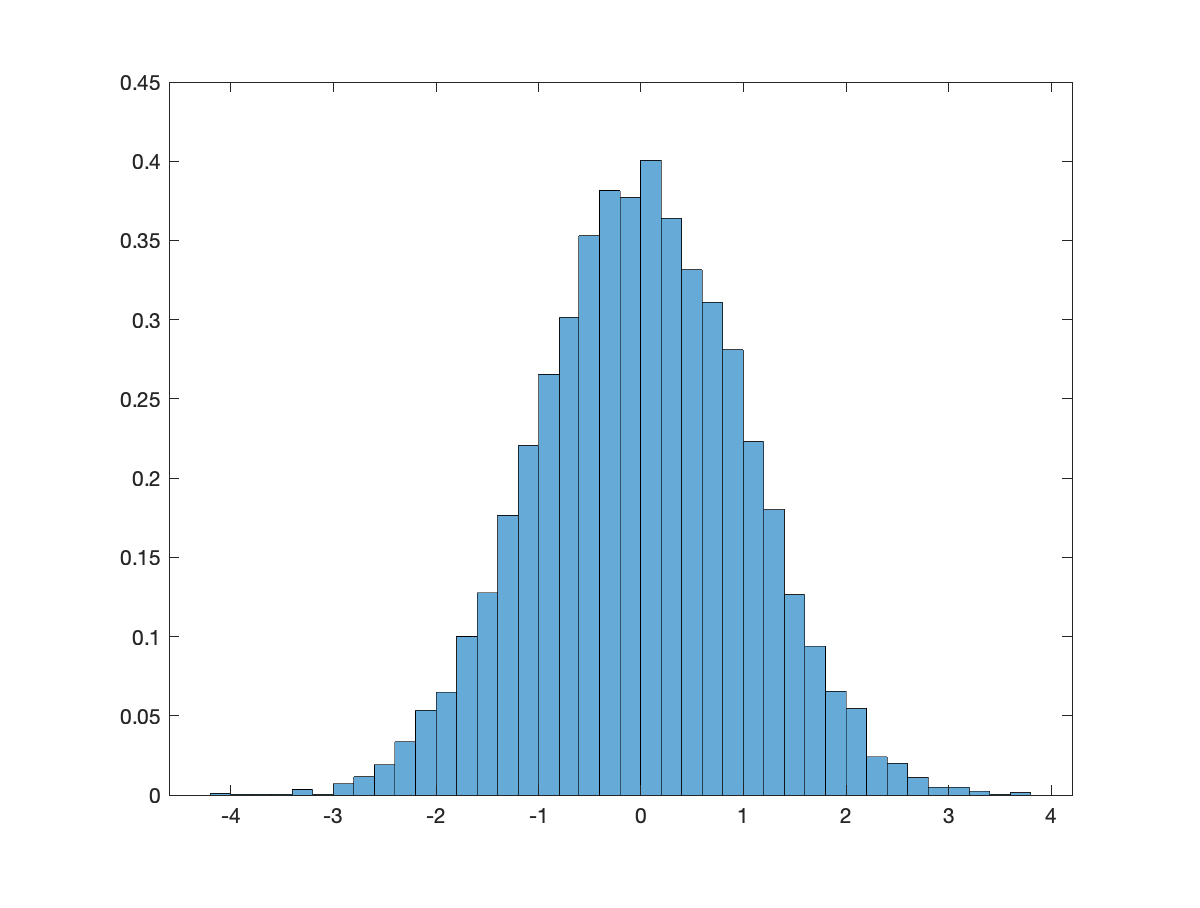
\includegraphics[width=12cm]{Image_8_25}
\caption{Test Data for Normal Distribution}\label{NormTest}
\end{figure}

To find a $100\alpha\%$ confidence interval we first must construct a pivot quantity. Suppose $X_{1},X_{2},\hdots,X_{n}\sim \Nd\left(\mu,\sigma^{2}\right)$ are independent and $\sigma^{2}$ is known. Note that $\overline{X}=\sum_{i}X_{i}/n\sim \Nd\left(\mu,\sigma^{2}/n\right)$ and so $Z=\sqrt{n/\sigma^{2}}\left(\overline{X}-\mu\right)\sim \Nd\left(0,1\right)$ for all $\mu$ and $\sigma^{2}$. If we take $\gamma_{\alpha}$ to equal the $(1+\alpha)/2$ upper quantile of a $\Nd\left(0,1\right)$ distribution then
\begin{equation}
\begin{aligned}
\alpha &= \mathbb{P}\left(-\gamma_{\alpha}\leq \sqrt{n/\sigma^{2}}\left(\overline{X}-\mu\right)\leq \gamma_{\alpha} \right)\\
&= \mathbb{P}\left(\overline{X}-\gamma_{\alpha}\sqrt{\sigma^{2}/n}\leq\mu\leq\overline{X}+\gamma_{\alpha}\sqrt{\sigma^{2}/n}\right)
\end{aligned}
\end{equation}
Hence we have a $100\alpha\%$ confidence interval for $\mu$: $\left[\overline{X}\pm\gamma_{\alpha}\sqrt{\sigma^{2}/n}\right]$. In the case of Question 10, we set $\sigma=1$ and $\gamma_{0.8}\approx1.2815516$ (the $90\%$ quantile of a standard normal variable). Our confidence interval then becomes 
\begin{equation}
\left[\overline{X}-\frac{1.2815516}{\sqrt{n}} \, , \, \overline{X}+\frac{1.2815516}{\sqrt{n}}\right]
\end{equation}
\subsection*{\centering Question 11}
When we set $n=100$, our confidence interval for $\mu$ becomes 
\begin{equation}
\left[ \overline{X}-0.12815516 \, , \, \overline{X}+0.12815516\right]
\end{equation}
\nameref{cd:11.1} referenced on page \pageref{cd:11.1} was used to generate Table \ref{tb:Q11} below. 
\begin{table}[H]
\centering
\begin{tabular}{|c|c|c|c|}
\hline $\overline{X}$ & Lower Bound for C.I. & Upper Bound for C.I. & True/False for interval\\
\hline -0.11141056385008 & -0.23956572040454 & 0.016744592704381 & 1\\ -0.097442634600331 & -0.22559779115479 & 0.030712521954129 & 1\\ -0.049409489376418 & -0.17756464593088 & 0.078745667178042 & 1\\ -0.065699270002723 & -0.19385442655718 & 0.062455886551737 & 1\\ 0.081887773925232 & -0.046267382629228 & 0.21004293047969 & 1\\ -0.023318872858958 & -0.15147402941342 & 0.1048362836955 & 1\\ -0.0038378606508644 & -0.13199301720532 & 0.1243172959036 & 1\\ -0.17261859581236 & -0.30077375236682 & -0.044463439257898 & 0\\ 0.053820604769822 & -0.074334551784638 & 0.18197576132428 & 1\\ -0.2112695160693 & -0.33942467262376 & -0.083114359514837 & 0\\ -0.0024082818682331 & -0.13056343842269 & 0.12574687468623 & 1\\ 0.090217072305278 & -0.037938084249182 & 0.21837222885974 & 1\\ 0.027318990321538 & -0.10083616623292 & 0.155474146876 & 1\\ 0.096422038106622 & -0.031733118447838 & 0.22457719466108 & 1\\ -0.091935809382862 & -0.22009096593732 & 0.036219347171598 & 1\\ 0.022751653259254 & -0.10540350329521 & 0.15090680981371 & 1\\ -0.11744730176472 & -0.24560245831918 & 0.01070785478974 & 1\\ 0.0022436660630844 & -0.12591149049138 & 0.13039882261754 & 1\\ -0.045793939331109 & -0.17394909588557 & 0.082361217223351 & 1\\ -0.027257261678682 & -0.15541241823314 & 0.10089789487578 & 1\\ -0.014931886796702 & -0.14308704335116 & 0.11322326975776 & 1\\ 0.17818514704297 & 0.050029990488512 & 0.30634030359743 & 0\\ 0.15136875657566 & 0.023213600021196 & 0.27952391313012 & 0\\ -0.13501257434764 & -0.2631677309021 & -0.0068574177931814 & 0\\ 0.18822715308006 & 0.060071996525596 & 0.31638230963452 & 0 \\ \hline
\multicolumn{3}{|r|}{Total} & 19\\ \hline
\end{tabular}
\caption{Confidence Intervals for Normal Variable}\label{tb:Q11}
\end{table}
There were 6 cases where the mean did not lie in the confidence interval. The expected number of times the mean would not lie in the confidence interval is $(1-0.8)\times 25=5$, so the value of 6 is reasonable.

\subsection*{\centering Question 12}
Using the general form of a $100\alpha\%$ confidence interval in Question 10 we see that changing $\mu$ has no effect, however changing $n$ does. If we keep the same interval $\left[\overline{X}\pm0.12815516\right]$ (the confidence interval for Question 11), when $n=50$ and $\mu=4$, then the new upper quantile $\gamma_{\widetilde{\alpha}}$ would equal $0.12815516\times\sqrt{50}=0.90619$. We calculate $\Phi\left(\gamma_{\widetilde{\alpha}}\right)=(1+\widetilde{\alpha})/2=0.81758$ (where $\Phi$ is the cumulative distribution function for a standard normal variable) and so $\widetilde{\alpha}=0.635167$. This implies that on average $(1-0.635)\times 25\approx 9$ cases will lie outside this confidence interval. This conclusion was tested by \nameref{cd:11.1}\footnote{The function \texttt{NormGenerate}, defined in Code 10.1, was used implicitly and has not been referenced at the end of this project.}, however lines 21 and 22:
\begin{verbatim}
Data(Counter,2)=sum(Variables)/n-norminv((1+alpha)/2)*sqrt(SigmaSquared/n);
Data(Counter,3)=sum(Variables)/n+norminv((1+alpha)/2)*sqrt(SigmaSquared/n);
\end{verbatim}
were replaced with:
\begin{verbatim}
Data(Counter,2)=sum(Variables)/n-0.12815516;
Data(Counter,3)=sum(Variables)/n+0.12815516;
\end{verbatim}
Using this modified code, the number of cases that lied outside the interval was calculated as 11, which is close to 9. This code was run 50 times and the average number of cases outside the interval was recorded as 9.36. This confirms the conclusion.

\subsection*{\centering Question 13}
We aim to prove that a $\chi_{n}^{2}$ distribution with $n$ degrees of freedom is the same as a $\Gamma\left(n/2,1/2\right)$ distribution. It is sufficient to prove the two moment generating functions of these distributions are the same in some non-zero interval around 0. From Question 4 we already know the m.g.f. of $Z\sim\Gamma\left(\alpha,\beta\right)$ is $\E{e^{-tZ}}=(1-t/\beta)^{-\alpha}$ for $t < \alpha$ and does not exist for $t\geq\alpha$. In the case $X\sim\chi_{n}^{2}$ we find $\E{e^{tX}}=\E{e^{tX_{1}^{2}+\hdots+tX_{n}^{2}}}$ where each $X_{i}\sim \Nd(0,1)$ are independent. Hence
\begin{equation}
\E{e^{tX}}=\prod_{i=1}^{n}\E{e^{tX_{i}^{2}}}=\left(\E{e^{tX_{1}^{2}}}\right)^{n}
\end{equation}
by independence. We know
\begin{equation}
\begin{aligned}
\E{e^{tX_{1}^{2}}} &=\int_{-\infty}^{\infty}\frac{1}{\sqrt{2\pi}}\exp\left(-\frac{1}{2}\left(1-2t\right)x^{2}\right)\mathrm{d}x\\
&= \sqrt{\frac{1}{1-2t}}\int_{-\infty}^{\infty}\frac{1}{\sqrt{2\pi}\sqrt{\left(1-2t\right)^{-1}}}\exp\left(-\frac{1}{2\left(1-2t\right)^{-1}}x^{2}\right)\mathrm{d}x\\
&=\sqrt{\frac{1}{1-2t}}
\end{aligned}
\end{equation}
provided $t<1/2$ (and does not exist for $t\geq 1/2$). Hence we deduce that the m.g.f. of a $\chi_{n}^{2}$ distribution is
\begin{equation}
\E{e^{tX}}=\left(\frac{1}{1-2t}\right)^{n/2}
\end{equation}
for $t<1/2$. This is identical to the m.g.f of the gamma distribution $\Gamma\left(n/2,1/2\right)$ in the interval $t\in(-1/2,1/2)$. We  conclude that these two distributions are the same and that the p.d.f of a $\chi_{n}^{2}$ distribution is
\begin{equation}\label{eq:PDF13}
\frac{x^{n/2-1}e^{-x/2}}{2^{n/2}\Gamma\left(n/2\right)}
\end{equation}
This exact solution has been plotted against the histograms below to better portray the shape of this distribution.\\
The following figures until the end of this report were produced by \nameref{cd:13.1}, referenced on page \pageref{cd:13.1}.\footnote{The function \texttt{NormGenerate}, defined in Code 10.1, was used implicitly here and has not been included in the reference.} Below are three plots of the estimated $\chi_{1}^{2}$ distribution with $n=100,300$ and $500$. 

\begin{figure}[H]
\centering
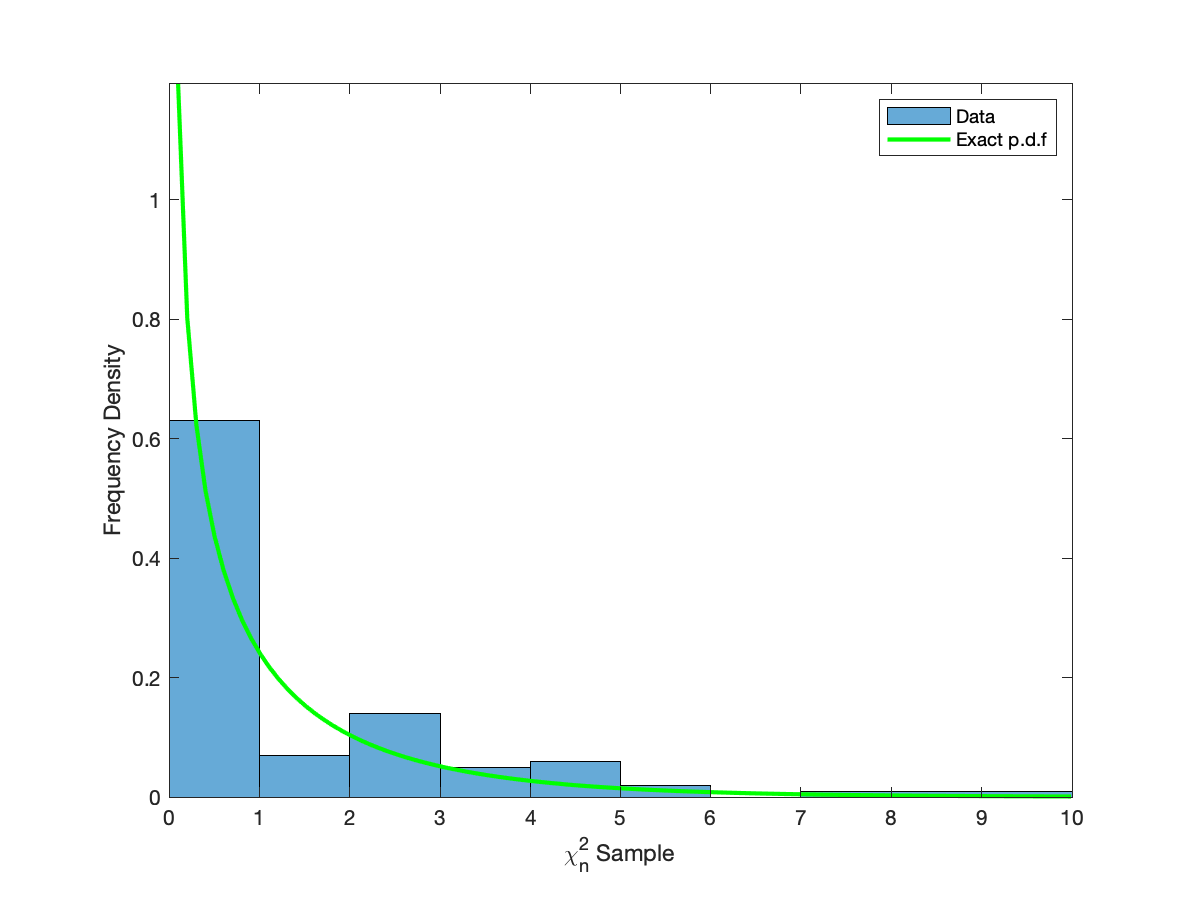
\includegraphics[width=10cm]{Image_13_1_1}
\caption{P.d.f. of $\chi_{1}^{2}$ distribution with $n=100$}\label{fg:13.1}
\end{figure}
\begin{figure}[H]
\centering
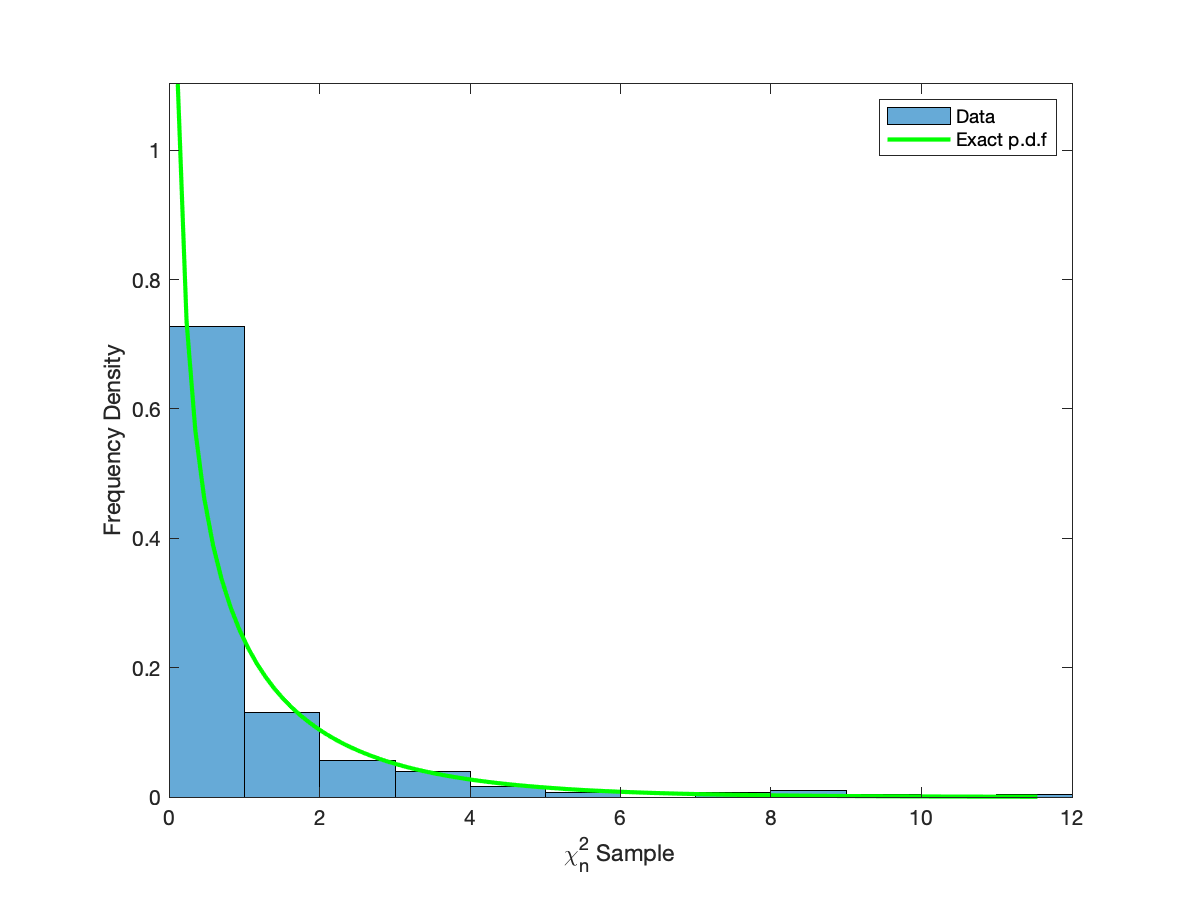
\includegraphics[width=10cm]{Image_13_1_2}
\caption{P.d.f. of $\chi_{1}^{2}$ distribution with $n=300$}
\end{figure}
\begin{figure}[H]
\centering
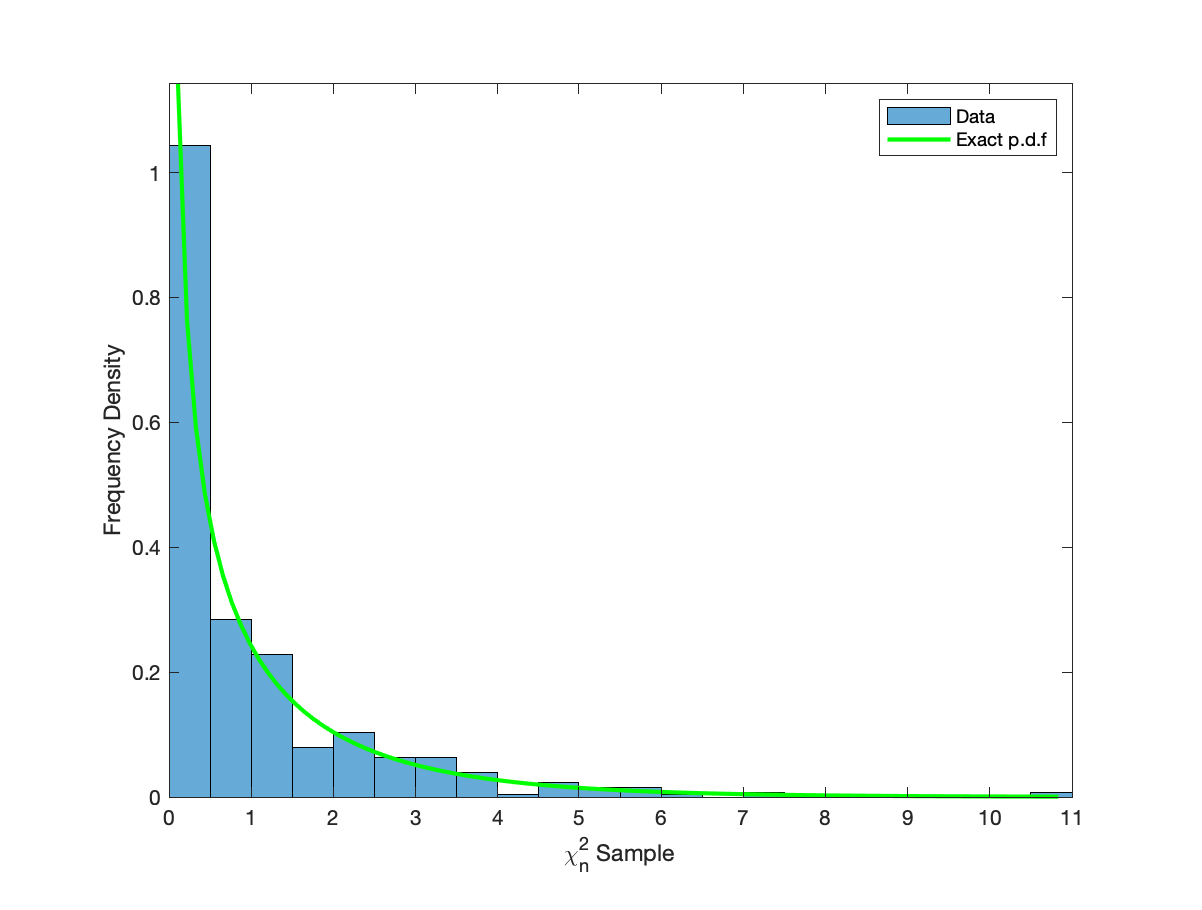
\includegraphics[width=10cm]{Image_13_1_3}
\caption{P.d.f. of $\chi_{1}^{2}$ distribution with $n=500$}
\end{figure}

We can see that as $n$ grows the approximation tends towards the analytic p.d.f.  This is because for a larger sample size, outliers do not effect the overall conclusion as much, and so our sample tends towards the exact distribution. Therefore when comparing how this distribution evolves with time we should set $n=500$ to be most accurate.  The following two figures are plots of the $\chi_{5}^{2}$ and $\chi_{40}^{2}$ when $n=500$.
\begin{figure}[H]
\centering
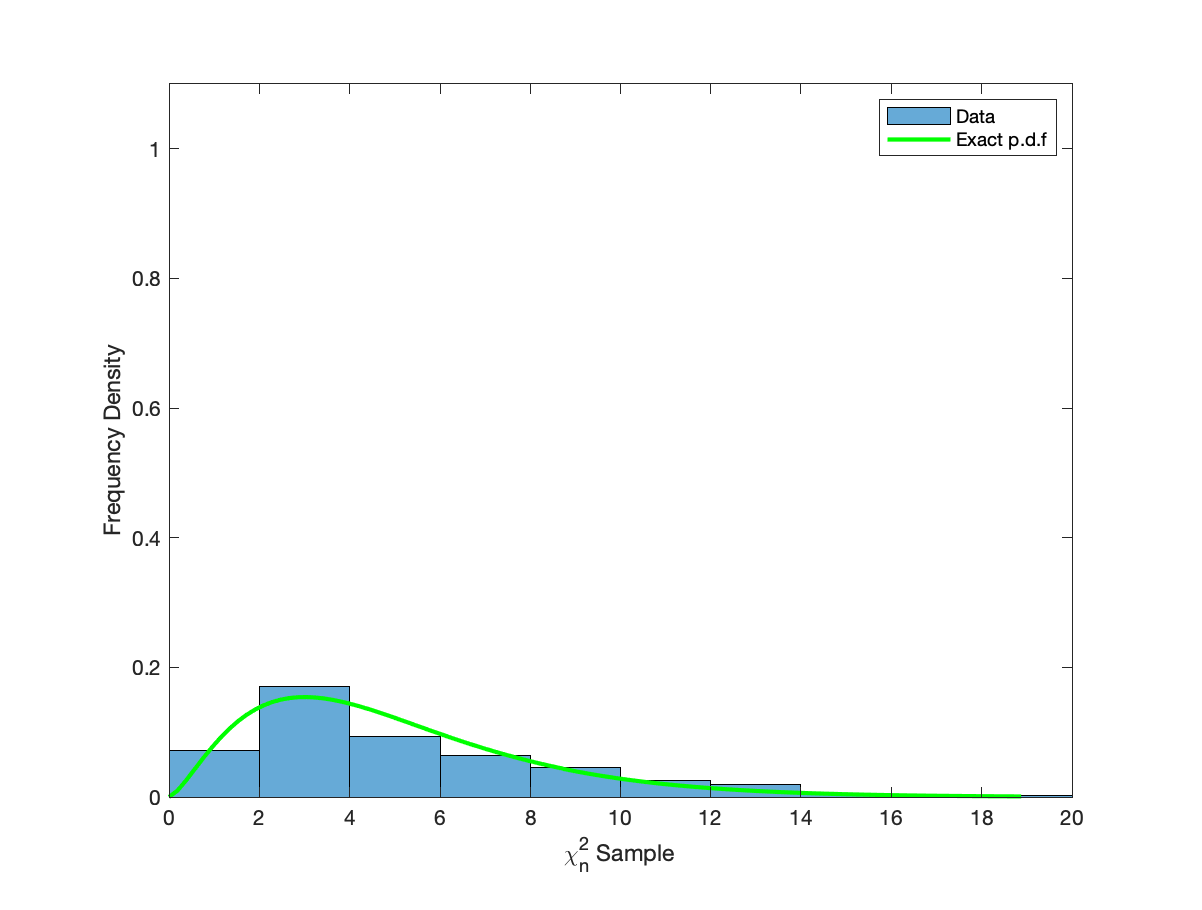
\includegraphics[width=10cm]{Image_13_2}
\caption{P.d.f. of $\chi_{5}^{2}$ distribution with $n=500$}
\end{figure}
\begin{figure}[H]
\centering
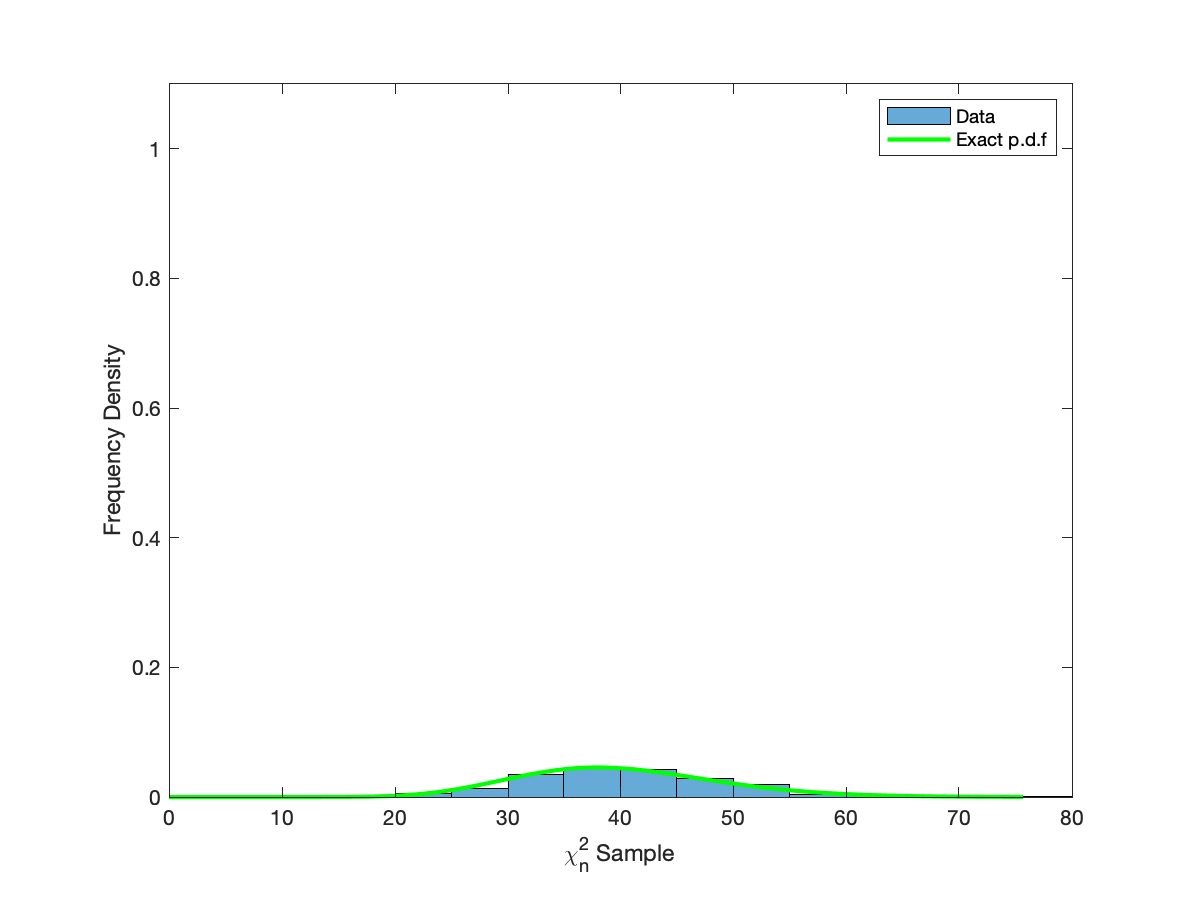
\includegraphics[width=10cm]{Image_13_3}
\caption{P.d.f. of $\chi_{40}^{2}$ distribution with $n=500$}
\end{figure}
Using the p.d.f. in equation \eqref{eq:PDF13}, we can deduce the expectation and variance of $X_{n}\sim \chi_{n}^{2}$ distribution:
\begin{equation}\label{eq:Q13E}
\begin{aligned}
\E{X_{n}} &=\frac{1}{2^{n/2}\Gamma\left(n/2\right)}\int_{0}^{\infty}x^{n/2}e^{-x/2}\mathrm{d}x\\
&=\frac{2\Gamma\left(n/2+1\right)}{\Gamma\left(n/2\right)}=n
\end{aligned}
\end{equation}
and 
\begin{equation}\label{eq:Q13Var}
\begin{aligned}
\Var{X_{n}} &=\frac{1}{2^{n/2}\Gamma\left(n/2\right)}\int_{0}^{\infty}x^{n/2+1}e^{-x/2}\mathrm{d}x-n^{2}\\
&=\frac{2\Gamma\left(n/2+2\right)}{\Gamma\left(n/2\right)}-n^{2} = 2n
\end{aligned}
\end{equation}
This makes sense in the figures above, since, as $n$ increases, we can see the distribution spreading out and shifting to the right. It also appears to be positively skewed, however it looks like it becomes more symmetrical as $n$ grows large. In fact we claim that the p.d.f approaches a $\Nd(n,2n)$ distribution. The proof comes from the central limit theorem; if $Y_{i}$ are independently distributed as the squares of standard normal variables with $\mu=\E{Y_{i}}$ and $\sigma^{2}=\Var{Y_{i}}$, then
\begin{equation}
\lim_{n\rightarrow \infty}\left(\sqrt{n}\frac{\frac{X_{n}}{n}-\mu}{\sqrt{\sigma^{2}}}\right)\xrightarrow{d}  Z
\end{equation}
where $Z\sim \Nd(0,1)$ and $X = \sum_{i}Y_{i}\sim\chi_{n}^{2}$. From equations \eqref{eq:Q13E} and \eqref{eq:Q13Var} we know $\mu=1$ and $\sigma^{2}=2$,  so $X\xrightarrow{d} \sqrt{n\sigma^{2}}Z+n\mu\sim \Nd(n,2n)$. This proves that the skewness and kurtosis (the measure of how heavily the tails of a distribution differ from that of a normal distribution) both tends to 0.\\
Also when $n=1$ or 2, the mode of this distribution is equal to 0, however for all other $n$ it is strictly positive. Also the only value of $n$ for which the p.d.f. is unbounded is $n=1$ (using equation \eqref{eq:PDF13}).

\section*{\centering References}\label{References}
\printbibliography[heading=none]

\pagebreak
\section*{\centering Code}
\subsection*{\centering Code 2.1}\label{cd:2.1}
\begin{verbatim}
n=[25,50,100];
dimN=size(n,2);
theta=1.2;
Legend=cell(dimN,1);

Counter=1;
figure
while Counter<=dimN
    Variables=zeros(n(Counter),3);
    Variables(:,1)=1:n(Counter);
    Variables(:,2)=rand(n(Counter),1);
    Variables(:,3)=-log(1-Variables(:,2))/theta;
    % disp(Variables)
    %Produces a latex table
    %latex(sym(vpa(Variables)))
    Max=log(2)*sum(Variables(:,3))/n(Counter);
    disp(Max)

    %Plots the log likelihood function
    m=linspace(0,5);
    y=loglike(Variables(:,3),m,n(Counter));
    plot(m,y)
    hold on
    Legend{Counter,1}=strcat('n=',num2str(n(Counter)));
    Counter=Counter+1;
end
xlabel("m")
ylabel("Log Likelihood function")
legend(Legend)
print('Image_3_4','-depsc')



%This calculates the log likelihood using the data x plotted against m
function answer=loglike(x,m,n)
    count=1;
    answer=1;
    while count<=n
        answer=answer.*g(x(count),m);
        count=count+1;
    end
    answer=log(answer);
end

%This is the p.d.f paramterised in terms of m
function answer=g(x,m)
    answer=log(2)./(m.*2.^(x./m));
end
\end{verbatim}
\pagebreak
\subsection*{\centering Code 7.1}\label{cd:7.1}
\begin{verbatim}
n=[10,30,50];
theta=2.2;

Counter=1;
mle=zeros(3,1);

figure
while Counter<=3
    u=rand(n(Counter),2);
    x=-log(1-u(:,1))/theta-log(1-u(:,2))/theta;
    %Produces a latex table
    %latex(sym(vpa(x)))
    mle(Counter)=2*n(Counter)/sum(x);

    %Plots the log likelihood function
    t=linspace(0,5);
    y=loglike(x,t,n(Counter));
    plot(t,y)
    hold on
    Counter=Counter+1;
end

xlabel("\theta")
ylabel("Log Likelihood Function")
legend('n=10','n=30','n=50')
print('Image_7_1','-depsc')

disp(mle)

function answer=loglike(x,t,n)
    count=1;
    answer=1;
    while count<=n
        answer=answer.*g(x(count),t);
        count=count+1;
    end
    answer=log(answer);
end

function answer=g(x,t)
    answer=t.^(2)*x.*exp(-t*x);
end
\end{verbatim}
\pagebreak
\subsection*{\centering Code 8.1}\label{cd:8.1}
\begin{verbatim}
n=[10,30,50];
theta=2.2;
Counter=1;
dimN=size(n,2);

MLEStats=zeros(dimN,3);

while Counter<=dimN
    %Calculates random variables for different sample sizes
    data=zeros(n(Counter),200);
    mle_data=zeros(1,200);
    count=1;
    while count<=200
        u=rand(n(Counter),2);
        x=-log(1-u(:,1))/theta-log(1-u(:,2))/theta;
        data(:,count)=x;
        mle_data(1,count)=2*n(Counter)/sum(x);
        count=count+1;
    end

    %Calculating Average and Varience in data
    MLEStats(Counter,1)=sum(mle_data)/200;
    var_mle=0;
    weight_var_mle=0;
    count=1;
    while count<=200
        var_mle=var_mle+(mle_data(1,count)-MLEStats(Counter,1))^2;
        weight_var_mle=weight_var_mle+(mle_data(1,count)-theta)^2;
        count=count+1;
    end
    MLEStats(Counter,2)=var_mle/200;
    MLEStats(Counter,3)=weight_var_mle/200;

    if Counter==1
        XLower=min(mle_data)-0.2;
        XHigher=max(mle_data)+0.2;
    end

    %Plots histogram with appropiate data
    figure
    histogram(mle_data,'Normalization','pdf')
    xlim([XLower,XHigher])
    hold on
    line([theta,theta],ylim,'LineWidth', 2,...
        'Color', 'r');
    hold on
    x=linspace(XLower,XHigher);
    y=pdf(x,2*n(Counter),theta);
    line(x,y,'LineWidth',2,'Color','g')

    legend('Data','\theta_{0}=2.2','Exact p.d.f','Location','northeast')
    xlabel('M.L.E')
    ylabel('Frequency Density')
    print(strcat('Image_8_',num2str(Counter)),'-depsc')

    Counter=Counter+1;
end
%MLE denotes average mle | Variance from average mle | Variance from 2.2
disp(MLEStats)
latex(sym(vpa(MLEStats)))

function answer = pdf(x,a,b)
    answer=(a*b)^(a)./((gamma(a)).*(x.^(a+1))).*exp(-b.*a./x);
end
\end{verbatim}
\pagebreak
\subsection*{\centering Code 10.1}\label{cd:10.1}
\begin{verbatim}
format shortg

Variables=NormGenerate(10000,0,1);
histogram(Variables,'Normalization','pdf')

function Variables = NormGenerate(n,mu,SigmaSquared)
    A=rand((n-mod(n,2))/2+mod(n,2),1);
    B=rand((n-mod(n,2))/2+mod(n,2),1);
    Phi=2*pi*A;
    V=-2*log(1-B);
    X=mu+SigmaSquared*sqrt(V).*cos(Phi);
    Y=mu+SigmaSquared*sqrt(V).*sin(Phi);
    Variables=[X;Y(1:n-(n-mod(n,2))/2-mod(n,2),1)];
end
\end{verbatim}
\pagebreak
\subsection*{\centering Code 11.1}\label{cd:11.1}
\begin{verbatim}
format shortg

%Set parameters
n=100;
mu=0;
SigmaSquared=1;
alpha=0.8;
SampleSize=25;

Counter=1;
Data=zeros(SampleSize,4);

disp([num2str(alpha),'% confidence interval is XBar plus or minus ',...
    num2str(norminv((1+alpha)/2)*sqrt(SigmaSquared/n))])

%Calculates random variables and fills table
while Counter<=SampleSize
    Variables=NormGenerate(n,mu,SigmaSquared);

    Data(Counter,1)=sum(Variables)/n;
    Data(Counter,2)=sum(Variables)/n-norminv((1+alpha)/2)*sqrt(SigmaSquared/n);
    Data(Counter,3)=sum(Variables)/n+norminv((1+alpha)/2)*sqrt(SigmaSquared/n);
    Data(Counter,4)=and(mu>=Data(Counter,2),mu<=Data(Counter,3));
    Counter=Counter+1;
end
disp(Data)
% latex(sym(vpa(Data)))

Out=SampleSize-sum(Data(:,4));
disp(['Number of cases outside interval: ',num2str(Out)])
\end{verbatim}
\pagebreak
\subsection*{\centering Code 13.1}\label{cd:13.1}
\begin{verbatim}
DoF=[1,5,40];
mu=0;
SigmaSquared=1;
SampleSize=100;

ChiData=zeros(SampleSize,1);
dimDoF=size(DoF,2);
Counter=1;
while Counter<=dimDoF

    %Calculates random varaibles by summing and squaring normal distributed
    %ones
    count=1;
    while count<= SampleSize
        n=DoF(Counter);
        Variables=NormGenerate(n,mu,SigmaSquared);
        ChiData(count,1)=dot(Variables,Variables);
        count=count+1;
    end
    %Plots histogram with distribution imposed
    figure
    histogram(ChiData,'Normalization','pdf')
    hold on
    x=linspace(0,max(ChiData));
    y=pdf(x,DoF(Counter)/2,1/2);
    line(x,y,'LineWidth',2,'Color','g')
    xlim([0,inf])
    ylim([0,1.1])
    legend('Data','Exact p.d.f','Location','northeast')
    xlabel('\chi^{2}_{n} Sample')
    ylabel('Frequency Density')
    print(strcat('Image_11_',num2str(Counter)),'-depsc')
    Counter=Counter+1;
end

function answer = pdf(x,a,b)
    answer=b^(a).*x.^(a-1).*exp(-b.*x)/gamma(a);
end
\end{verbatim}
\pagebreak

\end{document}